\documentclass[12pt]{beamer}
\usetheme{Warsaw}
\usepackage[utf8]{inputenc}
\usepackage{amsmath}
\usepackage{amsfonts}
\usepackage{amssymb}
\usepackage{graphicx}
\usepackage[font=Times,timeinterval=1,timeduration=2.0,timedeath=0,fillcolorwarningsecond=white!60!yellow,timewarningfirst=50,timewarningsecond=80,resetatpages=2]{tdclock}
\usepackage{tabularx}
\usepackage{array}
\usepackage{multicol}
\usepackage{longtable}
\usepackage{xcolor}
\usepackage{gensymb}
\usepackage{pgfplots}

\newcolumntype{Y}{>{\centering\arraybackslash}X}
\begin{document}
\begin{frame}
	\frametitle{Bellwork 8/22 (5 Minutes)}
	\initclock
	\textbf{[Piecewise-Defined Functions]}\vspace{.2cm}\\
	\vspace*{\fill}
	\begin{center}
		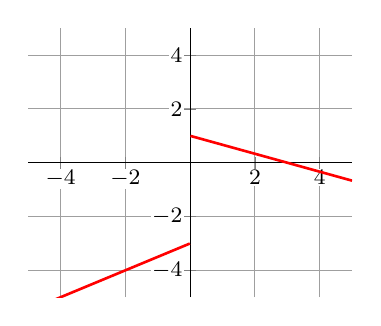
\begin{tikzpicture}[declare function={g(\x)=\x<0 ? 1/2*x-3 : (\x>0 ? -1/3*x+1 : inf);}]
			\begin{axis}[unbounded coords=jump,
					grid=both,
					grid style={line width=0.35pt, draw=gray!75},
					axis lines=center,
					axis line style={-},
					xmin=-5, xmax=5,
					ymin=-5, ymax=5,
					ticklabel style={font=\footnotesize,inner sep=0.5pt,fill=white,opacity=1.0, text opacity=1},
					every axis plot/.append style={line width=0.95pt, color=red, samples=500},
					scale=0.6
				]
				\addplot[samples at={-5,-0.01,0,0.01,5}] {g(x)};
			\end{axis}
		\end{tikzpicture}
	\end{center}
	\vspace*{\fill}
	\begin{center}
		Find a piecewise formula of this graph.\\
	\end{center}
	\vspace*{\fill}
	\vspace*{\fill}
	\crono
	\resetcrono{\beamerbutton{reset}}
\end{frame}
\begin{frame}
	\frametitle{Exercise}
	\vspace*{\fill}
	\vspace*{\fill}
	\initclock
	For each function, evaluate: \[\frac{f(a+h)-f(a)}{h}\]\\
	\begin{enumerate}
		\item $f(x) = x^2 + 3x$
		      \vspace*{\fill}
		\item $f(x) = x + 2$
		      \vspace*{\fill}
		\item $f(x) = 2x$
	\end{enumerate}
	\vspace*{\fill}
	\vspace*{\fill}
	\vspace*{\fill}
	\vspace*{\fill}
	\crono
	\resetcrono{\beamerbutton{reset}}
\end{frame}
\begin{frame}
	\frametitle{Exercise}
	\vspace*{\fill}
	\vspace*{\fill}
	\initclock
	Rewrite each function as a piecewise-defined one:\\
	\vspace*{\fill}
	\vspace*{\fill}
	\begin{enumerate}
		\item $f(x) = -|x+2|-3$
		      \vspace*{\fill}
		\item $g(x) = |1-x|$
		      \vspace*{\fill}
		\item $h(x) = 1-|x|$
	\end{enumerate}
	\vspace*{\fill}
	\vspace*{\fill}
	\vspace*{\fill}
	\vspace*{\fill}
	\crono
	\resetcrono{\beamerbutton{reset}}
\end{frame}
\begin{frame}
	\frametitle{Exercise}
	\vspace*{\fill}
	\vspace*{\fill}
	\vspace*{\fill}
	\initclock
	Determine whether each function is even, odd, or neither. Explain your reasoning.\\
	\vspace*{\fill}
	\begin{enumerate}
		\item $f(x) = x^4+x^2$
		\vspace*{\fill}
		\item $g(x) = -x^2+x$
		\vspace*{\fill}
		\item $h(x) = 2x^3+x$
	\end{enumerate}
	\vspace*{\fill}
	\vspace*{\fill}
	\vspace*{\fill}
	\vspace*{\fill}
	\crono
	\resetcrono{\beamerbutton{reset}}
\end{frame}
\end{document}